\documentclass{ximera}

\usepackage{todonotes}

\newcommand{\RR}{\mathbb R}
\renewcommand{\d}{\,d}
\newcommand{\dd}[2][]{\frac{d #1}{d #2}}
\renewcommand{\l}{\ell}
\newcommand{\ddx}{\frac{d}{dx}}
\newcommand{\dfn}{\textbf}
\newcommand{\eval}[1]{\bigg[ #1 \bigg]}
\renewcommand{\epsilon}{\varepsilon}
\newcommand{\p}[1]{\left(#1\right)}
\newcommand{\br}[1]{\left[#1\right]}
\newcommand{\set}[1]{\left\{#1\right\}}


\let\prelim\lim
\renewcommand{\lim}{\displaystyle\prelim}

\colorlet{textColor}{black} 
\colorlet{background}{white}
\colorlet{penColor}{blue!50!black} % Color of a curve in a plot
\colorlet{penColor2}{red!50!black}% Color of a curve in a plot
\colorlet{penColor3}{red!50!blue} % Color of a curve in a plot
\colorlet{penColor4}{green!50!black} % Color of a curve in a plot
\colorlet{penColor5}{orange!80!black} % Color of a curve in a plot
\colorlet{fill1}{blue!50!black!20} % Color of fill in a plot
\colorlet{fill2}{blue!10} % Color of fill in a plot
\colorlet{fillp}{fill1} % Color of positive area
\colorlet{filln}{red!50!black!20} % Color of negative area
\colorlet{gridColor}{gray!50} % Color of grid in a plot


\newcommand{\fullwidth}{}
\newcommand{\normalwidth}{}



%% makes a snazzy t-chart for evaluating functions
\newenvironment{tchart}{\rowcolors{2}{}{background!90!textColor}\array}{\endarray}


\author{Gregory Hartman \and Matthew Carr}
\license{Creative Commons 3.0 By-NC}
\acknowledgement{https://github.com/APEXCalculus}

\begin{document}
\begin{exercise}

\tag{derivative}

\outcome{Estimate the slope of the tangent line graphically.}
\outcome{Understand the derivative as a function related to the original function.}
\outcome{Combine derivative rules to take derivatives of more complicated functions.}

%% BADBAD approximation?


The graph of $f(x)=x^2-1$ is shown. 
	\begin{enumerate}
	\item		Use the graph to approximate the slope of the tangent line to $f$ at $(-1,0)$ and $(1,0)$.
	 \begin{enumerate}[label=\emph{(\roman*)}]
	  \item	 At $(-1,0)$, the slope of the tangent line to $f$ is approximately $\begin{prompt}\answer{-2}\end{prompt}$.
	  \item	 At $(1,0)$, the slope of the tangent line to $f$ is approximately $\begin{prompt}\answer{2}\end{prompt}$.
	 \end{enumerate}
	\item		Using the definition of the derivative, find $\ddx f(x)\begin{prompt} = \answer{2x}\end{prompt}$.
	\item		Find the slope of the tangent line at the points $(-1,0)$, $(0,-1)$ and $(2,3)$.
	\begin{enumerate}[label=\emph{(\roman*)}]
	  \item	 At $(-1,0)$, the slope of the tangent line to $f$ is exactly $\begin{prompt}\answer{-2}\end{prompt}$.
	  \item	 At $(1,0)$, the slope of the tangent line to $f$ is exactly $\begin{prompt}\answer{2}\end{prompt}$.
	  \item	 At $(2,3)$, the slope of the tangent line to $f$ is exactly $\begin{prompt}\answer{4}\end{prompt}$.
	 \end{enumerate}
	\end{enumerate}

\begin{center}
\noindent\begin{minipage}[t]{.5\linewidth}
 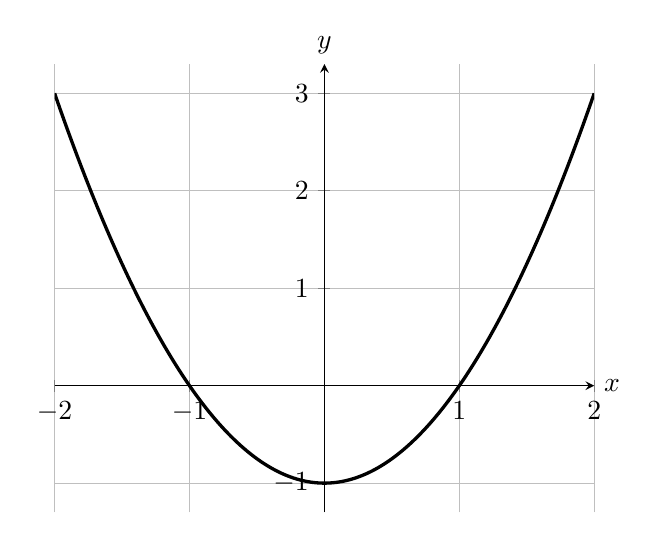
\begin{tikzpicture}
	\begin{axis}
	[ymin=-1.3,ymax=3.3, axis lines=center,xlabel=$x$,ylabel=$y$,every axis y 
	label/.style={at=(current axis.above origin),anchor=south},every axis x label/.style={at=(current axis.right of origin),anchor=west},
	domain=-2:2,
	ymajorgrids=true,
	grid = major
	]
	\addplot[domain=-2:2,very thick,smooth,samples=500]
	{pow(\x,2)-1};
	\end{axis}
       \end{tikzpicture}
\end{minipage}
\end{center}

\end{exercise}
\end{document}